\documentclass[12pt,letterpaper]{article}

\usepackage[letterpaper,margin=1.2in]{geometry}
\usepackage{fancyhdr}
\usepackage{lastpage}
\usepackage{graphicx}
\usepackage{csquotes}
\usepackage{url}
\usepackage{hyperref}
\usepackage{import}
\usepackage{color}
\usepackage[T1]{fontenc}
\usepackage{ragged2e}
\usepackage{verbatim}
\usepackage{listings}
\usepackage{multirow}
\definecolor{mygreen}{rgb}{0,0.6,0}
\definecolor{mygray}{rgb}{0.5,0.5,0.5}
\definecolor{mymauve}{rgb}{0.58,0,0.82}

\lstset{
    basicstyle=\scriptsize,
    numbers=left,
    numberstyle=\scriptsize,
    stepnumber=5,
    numbersep=5pt,
    showspaces=false, % don't show spaces by adding underscores
    showstringspaces=false, % don't underline spaces in strings
    showtabs=false, % don't show tabs with underscores
    frame=single,
    tabsize=4,
    captionpos=b,
    breaklines=true,
    breakatwhitespace=false,
    numberbychapter=false,
    stringstyle=\ttfamily %typewriter type for strings
      captionpos=b,                    % sets the caption-position to bottom
  commentstyle=\color{mygreen},    % comment style
  escapeinside={\%*}{*)},          % if you want to add LaTeX within your code
  keywordstyle=\color{blue},       % keyword style
  stringstyle=\color{mymauve},     % string literal style
}


\setlength{\headheight}{15pt}
\topmargin=-0.45in
\evensidemargin=0in
\oddsidemargin=0in
\textwidth=6.5in
\textheight=9.0in
\headsep=0.25in
\linespread{1.0}
\pagestyle{fancy}
\rhead{\AssShortTitle}
\lhead{\Class\ (\Instructor\ \Semster)}
\lfoot{}
\cfoot{\thepage}
\rfoot{}
\renewcommand\headrulewidth{0.4pt}
\renewcommand\footrulewidth{0.4pt}

\newcommand{\AssignmentTitle}{Assignment\ 7}
\newcommand{\Class}{CS532 Web Science}
\newcommand{\Instructor}{Dr. Michael L. Nelson}
\newcommand{\Semster}{- Spring 2016}
\newcommand{\AssShortTitle}{Assignment 7}
\newcommand{\MyName}{Naina Sai Tipparti}
\newcommand{\MyEmail}{ntippart@cs.odu.edu}

\setcounter{secnumdepth}{0}

\title{
\vspace{2in}
\textmd{\textbf{\Class:\ \AssignmentTitle}}\\
\normalsize\vspace{0.1in}\small{Finished on \today}\\
\vspace{0.1in}\large{\textit{\Instructor\ }}
\vspace{3in}
}

\hypersetup{colorlinks=true,
breaklinks=true,
urlcolor=blue,
linkcolor=black
}
\author{\textbf{\MyName} \\ \MyEmail}
\date{}

\begin{document}
\begin{titlepage}
\clearpage\maketitle
\thispagestyle{empty}
\end{titlepage}


\newpage
\clearpage
\tableofcontents
\lstlistoflistings
\listoftables
\thispagestyle{empty}
\justify
\section{Problem 1}

\subsection{Question}
\vspace*{10pt}
Write a Python program that extracts 1000 unique links from
Twitter.  You might want to take a look at:\\
\\
http://thomassileo.com/blog/2013/01/25/using-twitter-rest-api-v1-dot-1-with-python/\\
\\
But there are many other similar resources available on the web.  Note
that only Twitter API 1.1 is currently available; version 1 code will
no longer work.\\
\\
Also note that you need to verify that the final target URI (i.e., the
one that responds with a 200) is unique.  You could have many different
shortened URIs for www.cnn.com (t.co, bit.ly, goo.gl, etc.).\\
\\
You might want to use the search feature to find URIs, or you can
pull them from the feed of someone famous (e.g., Tim O'Reilly).\\
\\
Hold on to this collection -- we'll use it later throughout the semester.

\subsection{Answer}
\vspace{2mm}
Using the python module requests made this task a breeze as well as the initial code provided by Thomas Sileo's blog post.
\vspace{2mm}
\lstinputlisting[language=Python, caption=urifinder.py, label=listing:urifinder]{q1/urifinder.py}
\vspace{1mm}
The script was run multiple times to get the desired 1000 unique URIs. It would end prematurely at times, so the data set was initialized with the data of the previous run and then passed on to the {\tt find\_uris} function to preserve work performed.
\vspace{5mm}
\lstinputlisting[caption=Sample of 1000 Links, linerange=01-20]{q1/output.txt}

\section{Problem 2}
\label{problem2}
\subsection{Question}
\vspace*{10pt}
Write a Python program that:
\begin{enumerate}
\item takes as a command line argument a web page
\item extracts all the links from the page
\item lists all the links that result in PDF files, and prints out
      the bytes for each of the links.  (note: be sure to follow
      all the redirects until the link terminates with a "200 OK".)
\item show that the program works on 3 different URIs, one of which
needs to be:\\
http://www.cs.odu.edu/\~{}mln/teaching/cs532-s16/test/pdfs.html
\end{enumerate}
 
\subsection{Answer}
\vspace*{5mm}
In this python program, modules that are being used: 
\begin{enumerate}
\item Beautiful Soup is an HTML/XML parser for Python that can turn even invalid markup into a parse tree. It provides simple, idiomatic ways of navigating, searching, and modifying the parse tree. 
\\
\item Validators can be any callable that takes a single parameter which checks the new value before it is assigned to the attribute. Validators are permitted to modify a received value so that it is appropriate for the attribute definition. For example, using int as a validator will cast a correctly formatted string to a number, or raise an exception if it can not. However. the correct way to use a validator that ensure the correct type is to use the Type validator.
\\
\item Requests takes all of the work out of Python HTTP/1.1 — making your integration with web services seamless. There’s no need to manually add query strings to your URLs, or to form-encode your POST data. Keep-alive and HTTP connection pooling are 100\% automatic, powered by urllib3, which is embedded within Requests.
\end{enumerate}

\newpage
\vspace*{5pt}
\begin{center}
	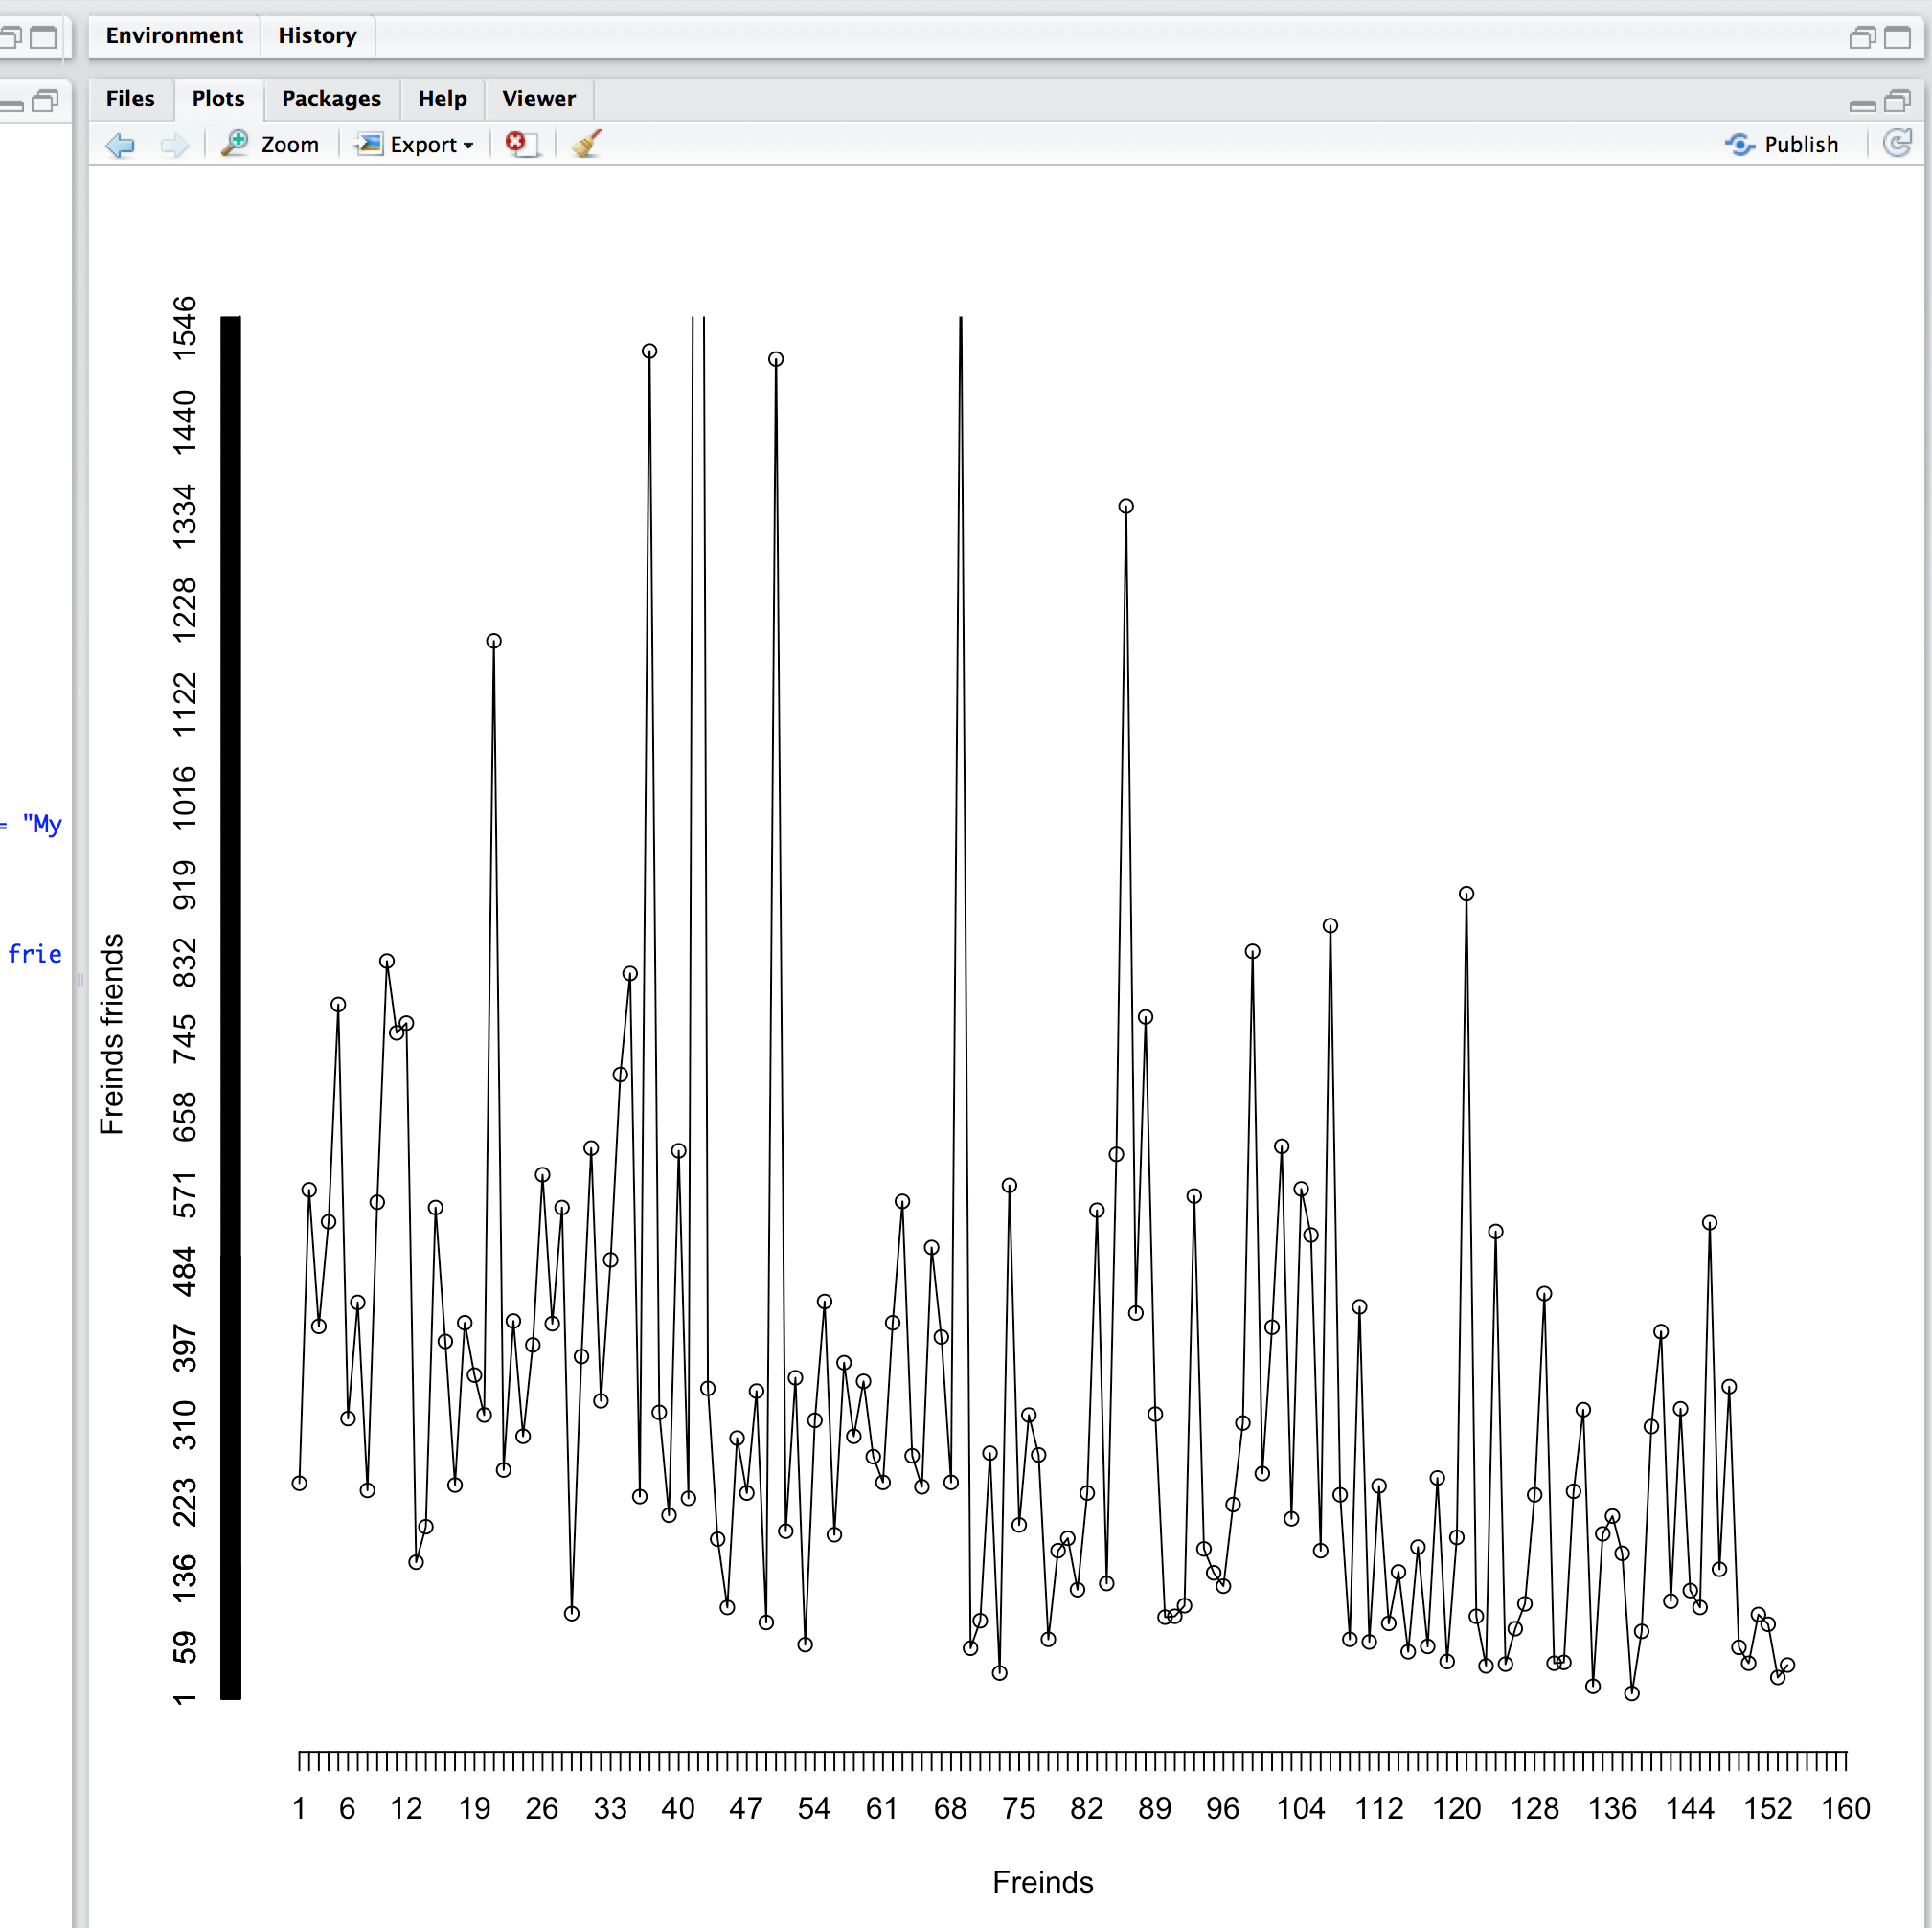
\includegraphics[scale=0.85]{Q2/fig1.png}
	\centerline{\textit{Figure 6: Output of q2.py at http://www.cs.odu.edu/\~{}mln/teaching/cs532-s16/test/pdfs.html
}}
\end{center}
\vspace*{5pt}
\begin{center}
	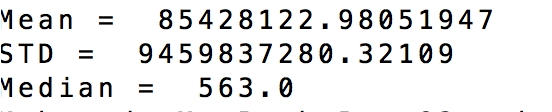
\includegraphics[scale=0.85]{Q2/fig2.png}
	\centerline{\textit{Figure 7: Output of q2.py at https://ws-dl.cs.odu.edu/Main/Pubs}}
\end{center}
\vspace*{5mm}
\begin{center}
	\includegraphics[scale=0.70]{Q2/fig3.png}
	\centerline{\textit{Figure 8: Output of q2.py at http://odu.edu/admission/graduate}}
\end{center}
Following python program $q2.py$, which accepts URL as argument and extracts PDF's from from the link:
\vspace*{1mm}

\begin{lstlisting}[frame = single,breaklines=true,numbers=left]
import sys
import requests
import validators
import locale
from urllib.parse import urlparse
from bs4 import BeautifulSoup

def main(url):
    print('\nExtracting all pdf links from: %s' % url)

    if requests.get(url).status_code != 200:
        print('\nURL not Found!\n')
        return
    page = requests.get(url).text
    url = 'http://' + urlparse(url).netloc
	
    soup = BeautifulSoup(page, 'html.parser')
    all_links = []
    for link in soup.find_all('a'):
        urls = link.get('href')
        if ((len(urls) > 6 and urls[:7].lower() != 'http://') 
        or len(urls) < 7) and urls[:8].lower() != 'https://':
            if urls[:2] == '//':
                urls = 'http:' + urls
            elif urls[0] != '/':    
                urls = url + '/' + urls
            else:
                urls = url + urls

        try:
            r = requests.get(urls)
            if 'Content-Type' in r.headers and 
            r.headers['Content-Type'] == 'application/pdf':
                if r.status_code == 200:
                    try:
                        all_links.append((urls, 
                        r.headers['Content-Length']))
                    except KeyError:
                        r.headers['Content-Length'] = '???'
                        all_links.append((urls, 
                        r.headers['Content-Length']))
        except requests.exceptions.SSLError:
            print('Couldn\'t open: %s. 
            URL requires authentication.' % urls)
        except requests.exceptions.ConnectionError:
            print('Couldn\'t open: %s. Connection refused.' % urls)
    print('\nList of all PDFs Links:')
    pdf_links = set(all_links)
    all_links = list(pdf_links)
    if len(all_links) > 0:
        for i in range(len(pdf_links)):
            if all_links[i][1] == '???':
                print('%s, File Size: %s bytes \n'
                 % (all_links[i][0], all_links[i][1]))
            else:
                print('%s, File Size: %s bytes \n' 
                % (all_links[i][0],                                  
                locale.format("%d", int(all_links[i][1]),
                grouping=True)))
    else:
        print('\nNo PDFs links for above URI.')
    return
if __name__ == '__main__':
    if len(sys.argv) != 2:
        print('\nUsage: python q2.py [url]')
        sys.exit(-1)
    if not validators.url(sys.argv[1]):
        print('URL is Invalid, Please try again')
        sys.exit(1)
    main(sys.argv[1])
    sys.exit(0)
\end{lstlisting}


\section{Problem 3}

\subsection{Question}
Compute the Kendall Tau\_b score for both lists (use \enquote{b} because
there will likely be tie values in the rankings).  Report both the
Tau value and the \enquote{p} value.\\
\\
See:\\ 
http://stackoverflow.com/questions/2557863/measures-of-association-in-r-kendalls-tau-b-and-tau-c\\
http://en.wikipedia.org/wiki/Kendall\_tau\_rank\_correlation\_coefficient\#Tau-b\\
http://en.wikipedia.org/wiki/Correlation\_and\_dependence\\



\subsection{Answer}
Using the Page Rank\cite{pagerank} Checker website to input each of the URIs found in the ten selected URIs from question 2 the results in Listing \ref{listing:pageranks} was determined.\\

\lstinputlisting[caption={page\_ranks file}, frame=none, stepnumber=0, label=listing:pageranks]{q3/page_ranks.txt}

In looking at the similarities and differences in the results of question 2 and question 3 it seems that page rank is unrelated to term frequency measurements. This is logical because the search term isn't taken as an input when calculating page rank. Also, finding page rank has a different goal than measuring search term relevance. It is used to objectively find which pages have a higher probability of a user randomly navigating to the page, which is unrelated to the content of the pages in the given set and is a function of the graph created by links contained in the pages of the set.
\section{Problem 4}

\subsection{Question}
\vspace*{10pt}
Determine if the friendship paradox holds for your Twitter account.
Since Twitter is a directed graph, use \enquote{followers} as value you measure 
$($i.e., \enquote{do your followers have more followers than you?}$)$.\\
\\
Generate the same graph as in question \#1, and calcuate the same 
mean, standard deviation, and median values.\\
\\
For the Twitter 1.1 API to help gather this data, see:
\\
\url{https://dev.twitter.com/docs/api/1.1/get/followers/list}
\\
If you do not have followers on Twitter (or don't have more than 50),
then use my twitter account \enquote{phonedude\_mln}.

\subsection{Answer}
Same instructions explained in question 2 are used to answer this question. As I remember, only one change has been made to {\it qet\_followers.py}. 
\\
\begin{itemize}
\item The old request:
\lstinputlisting[language=Python, linerange={73-73},stepnumber=0, caption={get\_followers.py}, label=listing:get_followers1]{q2/get_followers.py}
\item After modifying:
\lstinputlisting[language=Python,linerange={73-73},stepnumber=0, caption={get\_friends.py}, label=listing:get_friends]{q4/get_friends.py}
\end{itemize}
All new changes are stored in a new file called {\it qet\_friends.py}. The following is the output after running the Python program:
\vspace{2mm}
\begin{figure}[h!]
\centering
\fbox{\includegraphics[scale=0.65]{q4/fig3.png}}
\caption{Sample output of number of following}
\label{fig:number_following}
\end{figure}
\newpage
\vspace*{2mm}
\begin{table}
\centering
\begin{tabular}{ l l }
\hline
\textbf{Mean} & 484.9214 \\
\textbf{Median} & 225 \\
\textbf{Std Dev} & 729.5275\\
\hline
\end{tabular}
\caption{Statistics on the count of Dr.Nelson Following, values straight from R}
\label{tab:q4stats}
\end{table}
\begin{figure}[h!]
\centering
\fbox{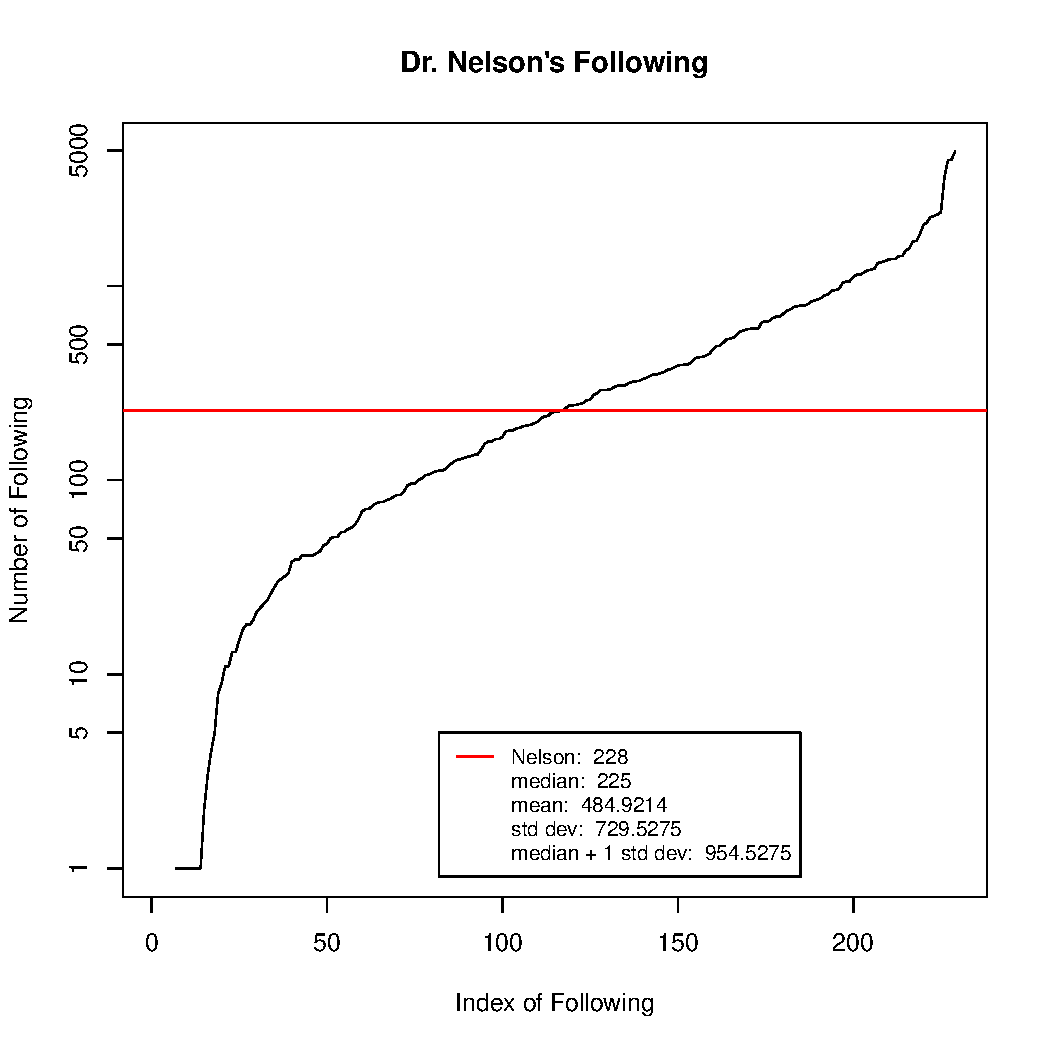
\includegraphics[scale=0.75]{q4/friend_plot.pdf}}
\caption{The Friendship Graph for Twitter Following}
\label{fig:followings_graph}
\end{figure}

I think here also the friendship paradox holds for Dr. Nelson Twitter account (for following) since the mean is equal to 484.9214 which greater than most of the number of following of Dr. Nelson following including himself. 
\section{Problem 5}

\subsection{Question}
Re-run question 2, but this time with proper TFIDF calculations instead of the hack discussed on slide 7 (p. 32).  Use the same 500 words, but this time replace their frequency count with TFIDF scores as computed in assignment \#3. Document the code, techniques, methods, etc. used to generate these TFIDF values.  Upload the new data file to github.\\
\\
Compare and contrast the resulting dendrogram with the dendrogram from question \#2.\\
\\
Note: ideally you would not reuse the same 500 terms and instead come up with TFIDF scores for all the terms and then choose the top 500 from that list, but I'm trying to limit the amount of work necessary.

\subsection{Answer}

To answer this question, {\tt matrix.py} was modified to add the capability to calculate {\it Term Frequency Inverse Document Frequency (TF/IDF)}. The added functions for computing TF/IDF are found in Listing \ref{listing:tfidf}. These functions use the master word count dictionary ({\tt wordcounts}) and each blog's individual word count ({\tt wc}) for each of the words in the {\tt wordlist} from Question 1/2 to compute the TF/IDF value for each word in the word list. 

\lstinputlisting[language=Python, caption={use of tfidf function},label=listing:tfidfmain,linerange={116-117},firstnumber=116]{matrix.py}

\lstinputlisting[language=Python, caption={writing the data}, label=listing:matrix:writedata, linerange={79-93}, firstnumber=79]{matrix.py}

\lstinputlisting[language=Python, caption={tf idf functions},label=listing:tfidf,linerange={40-48},
firstnumber=40]{matrix.py}

The same clustering was applied to the TF/IDF result matrix as was done in Question 2 and both images are displayed in Figures \ref{fig:raw} and \ref{fig:tfidf}.\\

There are a many pairs that were found to be similar in both clusterings. For example, in both dendrograms, the {\it Web Science and Digitial Libraries Research Group} blog is most similar to the {\it ...: zero pride and even less shame} blog, the {\it DJ DHANIEL FAN AND PRODUCER} is paired with {\it The Baron Boombox}, among a few others. In spite of this, the larger groupings do not appear very similar between the two clustings. There are some groups that share blogs in both dendrograms, but this is mostly due to there being only a few distinct groups in the raw count version and many of the TF/IDF clusters seemingly being subsets of the fewer, larger clustering from the raw count dendrogram.\\

When examining each of the clusters on a larger scale, it seems that the TF/IDF dendrogram clustered blogs are subjectively more alike than the raw count clusters. Looking toward the bottom of the TF/IDF clustering image, one will notice a grouping of blogs that seem closely related to music: {\it F-Measure: Less Than timely Music Reviews and Commentary.}, {\it Urban Anatomy's Columbian Jungle (That Dope!)} which seems to be a melding of fashion and music commentary, {\it Ezhevika Fields} a blog where info and preview samples of ``lost album samples of the past'' can be found, whereas these blogs are not all grouped together in the raw count dendrogram.\\

There is another cluster in the TF/IDF driven image that seems to contain family related blogs, with blogs like {\it Am I a funny girl?: I think I have my moments} which is, {\it The Frixen Family}, {\it When Two Hearts Become One: A wife, a mom, a daughter, a sibling.} and {\it The Clarks in Austin} all being related to a particular family and their everyday lives. Some of these blogs are close to each other in the raw count version, but they are not separated into their own distinct groups. The groups in the raw count version share some of these blogs, but are also mixed with others that seem unrelated. For example, the top cluster in the raw count dendrogram doesn't seem to have much of a unifying subject at all.\\

When looking at the overall structure of the two dendrograms it becomes apparent that there are more individual clusters grouped together in the TF/IDF version than are present in the raw count image, where there seems to be few small clusters and one mega-cluster in the center. This suggests that the TF/IDF algorithm was better at defining discrete subgroups within the larger context than the simple raw count dendrogram produced.

\begin{figure}[h!]
\centering
\fbox{\includegraphics[scale=0.3]{q2/blogclust.jpg}}
\caption{raw count dendrogram}
\label{fig:raw}
\end{figure}

\begin{figure}[h!]
\centering
\fbox{\includegraphics[scale=0.3]{q5/blogclust.jpg}}
\caption{TF/IDF dendrogram}
\label{fig:tfidf}
\end{figure}
\section{Problem 6}

\subsection{Question}
\vspace*{10pt}
Which 5 users are most correlated to the substitute you? Which
5 users are least correlated (i.e., negative correlation)?

\subsection{Answer}



\section{Appendix A}
\lstinputlisting[language=Python, caption={all code used}, label=listing:all]{recommendations.py}
\newpage
\vspace*{5pt}
\bibliographystyle{unsrt}
\bibliography{a7}
\end{document}
